\subsubsection{Descrizione generale}
Le classi \verb+ScoringService+ e \verb+BasicScoringService+ (che estende ScoringService\verb++) si occupano
del servizio di scoring di un post: \verb+ScoringService+ fornisce gli entry point per sfruttare 
i servizi Amazon AWS Comprehend\G{} e Rekognition\G, mentre è in \verb+BasicScoringService+ che sono 
implementate tutte le funzioni contenenti l'effettiva algoritmica di scoring e i servizi I/O.\\
Più nello specifico, \verb+ScoringService+ implementa:
\begin{lstlisting}[language=Python]
def __init__(self):
    self._rekognition = boto3.client(service_name='rekognition')
    self._comprehend = boto3.client(service_name='comprehend')
\end{lstlisting}
Che si occupa di fornire degli handles sotto forma di oggetti per accedere ai servizi AWS Rekognition\G{}
e Comprehend\G{} (\verb+self._rekognition+ e \verb+self._comprehend+).\\
\verb+BasicScoringService+ invece definisce e implementa le seguenti funzioni:

\begin{itemize}
\item 
\begin{lstlisting}[language=Python, numbers=none]
def process_event(self, event: ScoringEvent) -> dict:
\end{lstlisting}
Entry point per l'intera funzione di scoring, si occupa di lanciare tutti i servizi 
necessari a effettuare i vari scores e salva poi il risultato nel database. 
Ritorna infine una lista con tutti i post analizzati e i loro scores;

\item 
\begin{lstlisting}[language=Python, numbers=none]
def _save_to_db(self, db_post: models.Post, scoring_post: ScoringPost):
\end{lstlisting}
Salva nel database lo score assegnandolo ai relativi post;

\item 
\begin{lstlisting}[language=Python, numbers=none]
def _runRekognition(self, sPost: ScoringPost):
\end{lstlisting}
Lancia, tramite l'oggetto \verb+_rekognition+, le funzioni \verb+detect_text+ e 
\verb+detect_faces+ che si occupano di ritornare dei file JSON\G{} contenenti rispettivamente 
il testo a schermo (se presente) e una sentiment analysis dei volti (se presenti) 
dell'immagine di cui si vuole ottenere uno scoring. 
Dopodiché lancia \verb+__parse_rekognition_response+;

\item 
\begin{lstlisting}[language=Python, numbers=none]
def _runComprehend(self, sPost: ScoringPost):
\end{lstlisting}
Lancia, sfruttando l'oggetto \verb+_comprehend+ le funzioni \verb+detect_dominant_language+ 
e \verb+batch_detect_sentiment+, che si occupano rispettivamente di ritornare la lingua 
dominante di un documento e fornire una sentiment analysis di una lista di testi.
Dopodiché  lancia \verb+__parse_comprehend_response+;

\item 
\begin{lstlisting}[language=Python, numbers=none]
def _calcFinalScore(self, sPost: ScoringPost):
\end{lstlisting}
A seconda di quali scores siano presenti (caption, volti e testo a schermo), calcola 
lo score del post e lo salva in \verb+sPost.finalScore+;
   

\item 
\begin{lstlisting}[language=Python, numbers=none]
def __parse_rekognition_response(self, sPost: ScoringPost, textResult, faceResult):
\end{lstlisting}
Prende in input due file JSON\G{} (\verb+textResult+ e \verb+faceResult+), fa lo scoring dei volti 
ed estrapola 
da \verb+textResult+ (che contiene il testo rilevato dall'immagine) solo gli elementi 
di tipo \verb+"LINE"+, 
cioè quelli che contengono effettivamente il risultato voluto.
Salva poi i risultati in \verb+sPost.texts+ e \verb+sPost.faceScore+;

\item 
\begin{lstlisting}[language=Python, numbers=none]
def __parse_comprehend_response(self, sPost: ScoringPost, compResult):
\end{lstlisting}
Prende in input un file JSON\G{} contente i risultati delle sentiment analysis effettuate 
sulla caption e sul testo a schermo e ne effettua uno scoring che viene poi salvato 
in \verb+sPost.captionScore+ e \verb+sPost.textsScore+ (quest'ultima è in realtà una lista 
di scores dei vari frammenti di testo rilevati);

\item 
\begin{lstlisting}[language=Python, numbers=none]
def __parse_dominant_language_response(self, domResponse):
\end{lstlisting}
Ritorna il codice della lingua dominante, oppure \verb+'en'+ di default (cioè inglese);

\item 
\begin{lstlisting}[language=Python, numbers=none]
def __unpack_post_for_comprehend(self, sPost: ScoringPost)
\end{lstlisting}
Prepara il testo da fornire a Comprehend in modo che sia correttamente analizzato.
\end{itemize}
In linea generale lo scoring funziona come segue:
\verb+process_event+ chiama le funzioni \verb+_runRekognition+, \verb+_runComprehend+,
\verb+_calcFinalScore+ e \verb+_save_to_db+.\\
\verb+_runRekognition+ riconosce il testo a schermo ed effettua uno scoring dei volti;\\
\verb+_runComprehend+ effettua uno scoring del testo a schermo e della caption;\\
\verb+_calcFinalScore+ somma, secondo un certo criterio, i vari scores per ottenere lo score
finale del post, che viene quindi salvato nel corrispettivo post nel database da \verb+_save_to_db+.
\newpage
\subsubsection{Diagramma delle classi}
\begin{figure}[!h]
    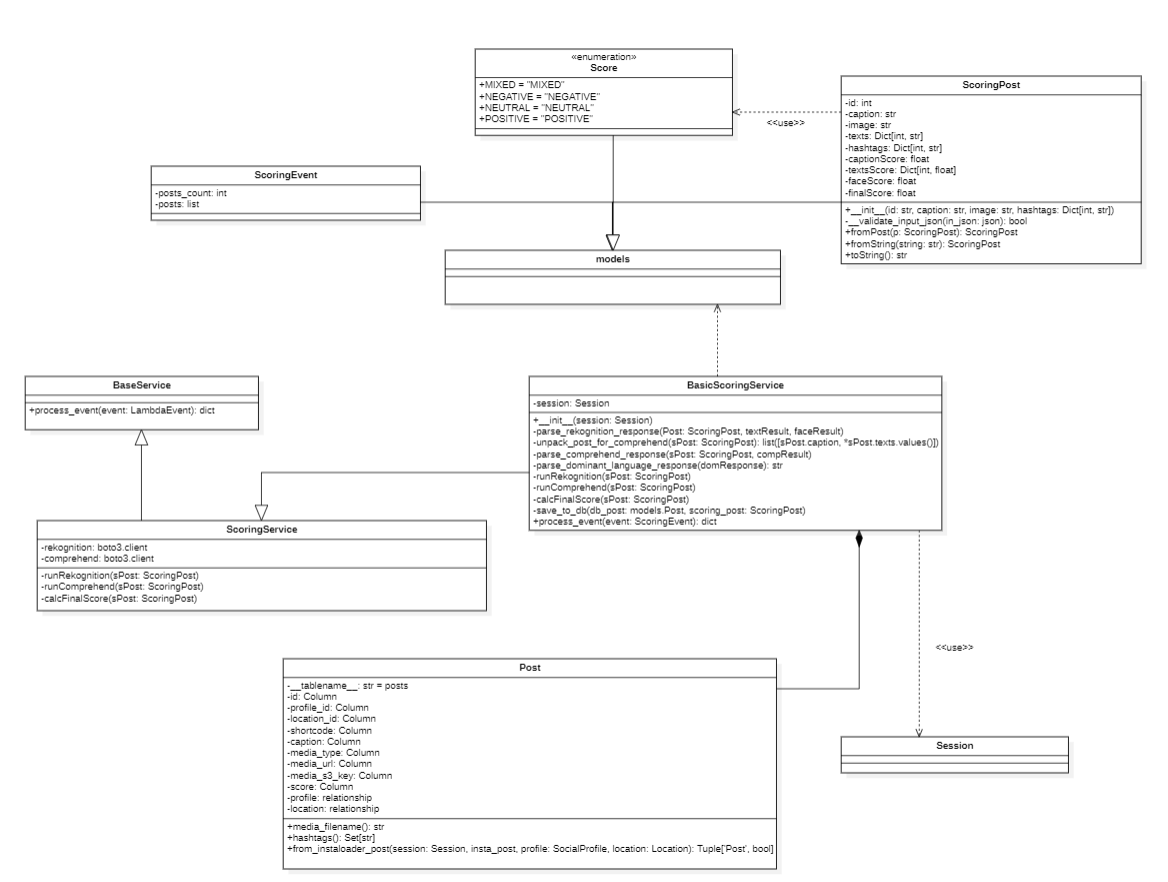
\includegraphics[width=15cm]{sezioni/images/cd_scoring.png}
    \caption{Scoring Service - Diagramma delle classi}
\end{figure}
\newpage
\subsubsection{Diagramma di sequenza}
\begin{figure}[!h]
    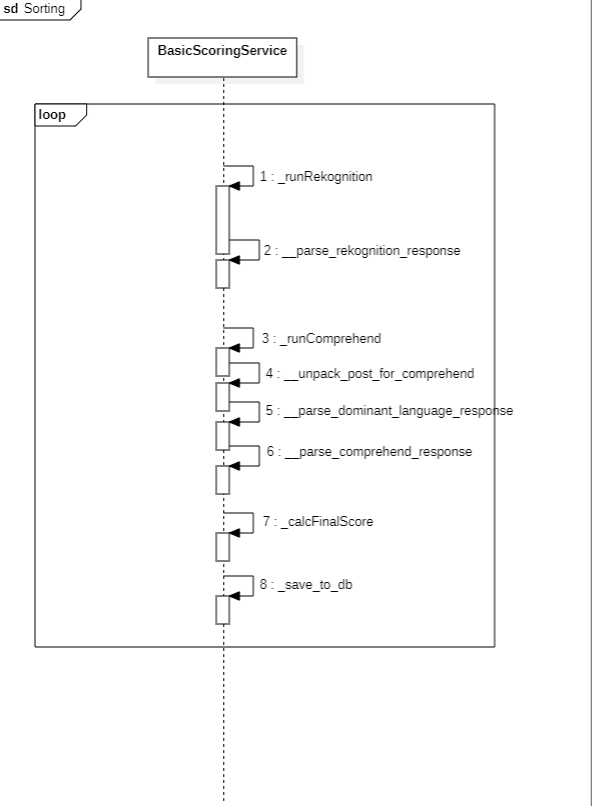
\includegraphics[width=15cm]{sezioni/images/sd_scoring.png}
    \caption{Scoring Service - Diagramma delle classi}
\end{figure}
\subsubsection{Schemi I/O}
\paragraph*{Input} esempio di evento in input, in formato JSON\G{}.
\begin{lstlisting}[language=JSON]
{
    "posts_count": 2,
    "posts": [
        {"id": 4},
        {"id": 5}
    ]
}
\end{lstlisting}
Descrizione:
\begin{itemize}
    \item \verb|posts_count|: numero di post di cui effetture lo scoring;
    \item \verb|posts|: array di post. 
\end{itemize}

\paragraph*{Output} esempio di risposta in output, in formato JSON\G{}.
\begin{lstlisting}[language=JSON]
{
    "scored_posts_count": 8,
    "scored_posts": [
        {
            "id": 4,
            "score": 4.830453701069928
        },
        {
            "id": 5,
            "score": 2.562992335879244
        },
    ]
}
\end{lstlisting}
Descrizione:
\begin{itemize}
    \item \verb|scored_posts_count|: numero di post di cui è stato effettuato lo score;
    \item \verb|scored_posts|: array di post con relativo score ottenuto. 
\end{itemize}

\subsubsection{Calcolo degli Scores}
Segue una spiegazione più dettagliata degli algoritmi e delle funzioni che si occupano di calcolare
i quattro scores necessari (\verb+faceScore+, \verb+textScore+, \verb+captionScore+, \verb+finalScore+).

\paragraph{faceScore} \aCapo
Il punto di partenza si trova nella funzione \verb+BasicScoringService._runRekognition+:
\begin{lstlisting}[language=Python]
Image = {
    'S3Object': {
        'Bucket': os.environ['ENV_BUCKET_NAME'],
        'Name': sPost.image,
    }
}
textResponse = self._rekognition.detect_text(Image=Image)
faceResponse = self._rekognition.detect_faces(Image=Image)
BasicScoringService.__parse_rekognition_response(
    sPost, textResponse, faceResponse
)
\end{lstlisting}
La variabile \verb+faceResponse+ contiene il risultato della funzionalità
di Rekognition\G{} chiamata \verb+detect_faces+ che prende in input un'immagine contenuta
in un bucket\G{} S3 e ritorna un file JSON\G{} contente una sentiment analysis dei vari volti presenti.\\
Segue un esempio del file in questione (lasciando implicito ciò che non serve):
\begin{lstlisting}[language=JSON]
{
"FaceDetails": [
    {
        "BoundingBox": {},
        "AgeRange": {},
        "Smile": {},
        "Eyeglasses": {},
        "Sunglasses": {},
        "Gender": {},
        "Beard": {},
        "Mustache": {},
        "EyesOpen": {},
        "MouthOpen": {},
        "Emotions": [
            {
                "Type": "ANGRY",
                "Confidence": 55.18563461303711
            },
            {
                "Type": "HAPPY",
                "Confidence": 37.01131820678711
            },{},{},{},{},{},{}
        ],
        "Landmarks": [],
        "Pose": {
            "Roll": 3.602341890335083,
            "Yaw": -82.46586608886719,
            "Pitch": -18.774751663208008
        },
        "Quality": {
            "Brightness": 92.66178894042969,
            "Sharpness": 9.912903785705566
        },
        "Confidence": 99.85897064208984
    }
}
\end{lstlisting}
Il risultato (contenuto in \verb+faceResponse+), viene quindi passato come parametro alla funzione 
\verb+BasicScoringService.__parse_rekognition_response+ che si occupa di effettuare il vero
e proprio scoring.\\
I valori (contenuti in \verb+FaceDetails+) che ci interessano sono:
\begin{itemize}
    \item Emotions: \begin{itemize}
        \item HAPPY
        \item CALM
        \item DISGUSTED \end{itemize}
    \item Pose: \begin{itemize}
        \item Yaw
        \item Pitch \end{itemize}
\end{itemize}
\verb+Quality+ non è necessario poiché, tramite testing, abbiamo notato che immagini con valori di 
\verb+Sharpness+ anche molto bassi vengono analizzate senza alcun problema. L'algoritmo perde precisione
solo nel caso in cui i volti siano ripresi da angolazioni troppo elevate (ad esempio da di lato).\\
Per quanto riguarda il campo \verb+Confidence+ delle \verb+Emotions+ può essere letto come una
"quantità di emozione" compresa tra 0 e 100 (la somma di tutti i valori di \verb+Confidence+ è uguale a 100):
in pratica una persona completamente felice avrà una \verb+Confidence+ dell'emozione \verb+HAPPY+ pari a 100 
(e tutte le altre pari a 0), mentre una persona completamente arrabbiata avrà una \verb+Confidence+ 
dell'emozione \verb+ANGRY+ pari a 100 (e tutte le altre pari a 0) e così via.\\
Segue la formula dello score dei volti in linguaggio semi-naturale:
\begin{lstlisting}
loop for all volti{
    if(volto dritto){
        score_volto = confidence_HAPPY + (confidence_CALM * 0.5)
        if(confidence_DISGUSTED too high){
            score_volto = 0
        }
    }
}
score_immagine_finale = somma_score_volti_dritti / numero_volti_dritti
\end{lstlisting}
Segue ora l'algoritmo: 
\begin{lstlisting}[language=Python]
faceCount = 0
scoreSum = 0
if len(faceResult['FaceDetails']) > 0:
    for face in faceResult['FaceDetails']:
        pose = face['Pose']
        # SE VOLTO DRITTO
        if (abs(pose['Yaw']) <= 50) and (
            abs(pose['Pitch']) <= 50
        ):  # abs() perche' deve essere -50<pose<50
            # CALCOLARE SCORE EMOZIONI
            faceCount = faceCount + 1
            faceSum = 0
            disgusted = False
            for emotion in face['Emotions']:
                if emotion['Type'] == 'HAPPY':
                    faceSum = faceSum + emotion['Confidence']
                if emotion['Type'] == 'CALM':
                    faceSum = (
                        faceSum + emotion['Confidence'] * 0.5
                    )  # ha peso minore di happy
                if emotion['Type'] == 'DISGUSTED':
                    if (
                        emotion['Confidence'] >= 50
                    ):  # se disgust troppo elevato azzera il punteggio 
                        #                                  della faccia
                        disgusted = True
            if not disgusted: 
                scoreSum = (
                    scoreSum + faceSum
                )  
        # UN VOLTO STORTO VIENE IGNORATO NEL CALCOLO
    faceScore = scoreSum / faceCount   # =[0,100]
    sPost.faceScore = faceScore / 100  # normalizzato a [0,1]
else:
    sPost.faceScore = None  # se num facce =0 si ignora nel calcolo 
                            #                        di final Score 
\end{lstlisting}
Il motivo per il quale \verb+CALM+ viene moltiplicato $*0.5$ è per dargli, nel calcolo del punteggio, un
peso pari alla metà di \verb+HAPPY+.\\
Infatti certamente non è un sentiment negativo, e va quindi
valutato positivamente, però è anche vero che deve valere meno di \verb+HAPPY+.\\
Il controllo riguardante l'angolazione del volto (cioè se il volto sia dritto o meno) viene
effettuato dal codice:
\begin{lstlisting}[language=Python]
if (abs(pose['Yaw']) <= 50) and (
    abs(pose['Pitch']) <= 50
):
\end{lstlisting}
Che controlla i valori d'imbardata e beccheggio del volto (in parole più semplici: \verb+Yaw+ è 
la rotazione della testa sull'asse perpendicolare al terreno, \verb+Pitch+ invece dell'asse parallelo al 
terreno e passante per le orecchie). \\
Si è scelto arbitrariamente il valore massimo di 50 e minimo 
di -50 per entrambi i valori al fine di evitare possibili errori: abbiamo riscontrato analisi del 
sentiment corrette anche con valori leggermente superiori, tuttavia è stata data maggiore priorità
all'affidabilità dell'analisi. \\
La parte riguardante l'emozione \verb+DISGUSTED+ è stata inserita perché ci è sembrato limitante usare
solo le emozioni \verb+HAPPY+ e \verb+CALM+ per dare una valutazione, soprattutto considerando che il tema
generale del progetto riguarda ristoranti e locali. Abbiamo quindi ritenuto
fondamentale dare il giusto peso a un'emozione così negativa. \\
Infatti un volto che abbia una
valutazione di \verb+DISGUSTED+$\geq50$ riceve uno score pari a 0. \\
Senza questo controllo sarebbe teoricamente
possibile che \verb+HAPPY+ fosse pari a 50 (contemporaneamente a \verb+DISGUSTED+=50) e quindi che lo score 
del volto fosse 50 su 100.
\begin{lstlisting}[language=Python]
    if emotion['Type'] == 'DISGUSTED':
        if (
            emotion['Confidence'] >= 50
        ): 
            disgusted = True
# end of for
if not disgusted:
scoreSum = (
    scoreSum + faceSum
)  # se volto disgusted value >=50 allora face value = 0
\end{lstlisting}
Come si vede dal codice soprastante, durante il ciclo che "scorre" i vari volti presenti viene
controllato il valore di \verb+DISGUSTED+ e, in caso sia superiore a 50, viene attivato un semaforo 
che impedisce di aggiungere lo score del volto alla somma generale (di fatto rendendo il valore
di suddetto volto pari a zero).\\
Vediamo quindi la parte terminale dell'algoritmo, che si occupa di salvare il \verb+faceScore+ vero e proprio:
\begin{lstlisting}[language=Python]
#if len(faceResult['FaceDetails']) > 0: 
# corpo dell' algoritmo 
    faceScore = scoreSum / faceCount 
    sPost.faceScore = faceScore / 100  # normalizzato a [0,1]
else:
    sPost.faceScore = None
\end{lstlisting}
Notiamo che \verb+faceScore+ viene calcolato come la media degli scores dei singoli volti, e viene poi
normalizzato. \\
Infatti gli scores sono compresi tra 0 e 100, ma è comodo avere lo score finale compreso
tra 0 e 1 (tornerà utile nel calcolo dello score finale). \\
Viene poi salvato in \verb+sPost.faceScore+. \\
Se non sono presenti volti viene assegnato allo score il valore di controllo \verb+None+.

\paragraph{textScore} \aCapo
Il punto di partenza si trova nella funzione \verb+BasicScoringService._runRekognition+:
\begin{lstlisting}[language=Python]
Image = {
    'S3Object': {
        'Bucket': os.environ['ENV_BUCKET_NAME'],
        'Name': sPost.image,
    }
}
textResponse = self._rekognition.detect_text(Image=Image)
faceResponse = self._rekognition.detect_faces(Image=Image)
BasicScoringService.__parse_rekognition_response(
    sPost, textResponse, faceResponse
)
\end{lstlisting}
La variabile \verb+textResponse+ contiene il risultato della funzionalità
di Rekognition\G{} chiamata \verb+detect_text+ che prende in input un'immagine contenuta
in un bucket\G{} S3 e ritorna un file JSON\G{} contente il testo presente nell'immagine.\\
Segue un esempio del file in questione (lasciando implicito ciò che non serve):
\begin{lstlisting}[language=JSON]
{
"TextDetections": [
    {
        "DetectedText": "PIZZA LAB",
        "Type": "LINE",
        "Id": 0,
        "Confidence": 99.8796615600586,
        "Geometry": {}
    },
    {
        "DetectedText": "Buon Ferragasta",
        "Type": "LINE",
        "Id": 1,
        "Confidence": 67.9867935180664,
        "Geometry": {}
    },{},{},{}
    ],
    "TextModelVersion": "3.0"
}        
\end{lstlisting}
Ciò che andremo a considerare in questo caso sarà il contenuto di \verb+DetectedText+
per ogni elemento di tipo \verb+LINE+.\\
Vediamo il codice: 
\begin{lstlisting}[language=Python]
for line in textResult['TextDetections']:
    if line['Type'] == 'LINE':
        sPost.texts[line['Id']] = line['DetectedText']
\end{lstlisting}
Ogni "pezzo" di testo rilevato nell'immagine viene salvato in un dizionario e viene
identificato dal suo \verb+Id+. Il dizionario in
questione è \verb+sPost.texts+.\\
Rispetto al JSON\G{} di esempio di cui sopra, il risultato di \verb+sPost.texts+ sarebbe il seguente:
\begin{lstlisting}[language=JSON]
{
    0: 'PIZZA LAB', 
    1: 'Buon Ferragasta'
}
\end{lstlisting}
A questo punto è Comprehend\G{} che deve occuparsi di dare degli effettivi sentiment
scores a queste stringhe di testo.\\
Il punto di partenza si trova nella funzione \verb+BasicScoringService._runComprehend+:
\begin{lstlisting}[language=Python]
dominantLanguageResponse = self._comprehend.detect_dominant_language(
    Text=sPost.caption
)
response = self._comprehend.batch_detect_sentiment(
    TextList=BasicScoringService.__unpack_post_for_comprehend(sPost),
    LanguageCode=BasicScoringService.__parse_dominant_language_response(
        dominantLanguageResponse
    ),
)
BasicScoringService.__parse_comprehend_response(sPost, response)
\end{lstlisting}
Ciò che interessa a noi è la variabile \verb+TextList+, ritornata dalla funzione \verb+__unpack+ 
(la variabile \verb+LanguageCode+ infatti è semplicemente una stringa che indica la lingua dominante della caption).\\
\verb+TextList+ infatti contiene sia la caption che la lista di testi rilevati a schermo, uniti in un
unica variabile dalla funzione \verb+__unpack+:
\begin{lstlisting}[language=Python]
def __unpack_post_for_comprehend(self, sPost: ScoringPost):
    if not sPost.caption:
        sPost.caption = ' '  
    return list([sPost.caption, *sPost.texts.values()])
\end{lstlisting}
Se la caption è un file vuoto la sostituisce con uno spazio, così da renderla accettabile in input
da Comprehend\G, e il risultato della funzione (cioè quindi ciò su cui viene lanciata la funzione di
sentiment detection di Comprehend\G) è il seguente (sempre prendendo ad esempio i file di cui sopra):
\begin{lstlisting}[language=JSON]
TextList = [
    'Caption',
    'PIZZA LAB',
    'Buon Ferragasta'
]
\end{lstlisting}
\verb+TextList+ viene quindi inoltrata a Comprehend\G tramite l'oggetto \verb+_comprehend+ e la sua
funzione \verb+batch_detect_sentiment+, che ritorna nella variabile \verb+response+ un file JSON\G{}
contenete la sentiment analysis per i vari pezzi di testo.\\
L'output di Comprehend\G è strutturato come segue:
\begin{lstlisting}[language=JSON]
{
    'ResultList': [
        {
            'Index': 0, 
            'Sentiment': 'POSITIVE', 
            'SentimentScore': {
                'Positive': 0.9763978719711304, 
                'Negative': 9.167650568997487e-05, 
                'Neutral': 0.02348191849887371, 
                'Mixed': 2.8541926440084353e-05
                }
        }, {}, {}
    ], 
    'ErrorList': [], 
    'ResponseMetadata': {}
}
\end{lstlisting}
Anche in questo caso lo scoring vero e proprio avviene nella funzione di parsing, vediamo quindi
l'algoritmo di scoring:
\begin{lstlisting}[language=Python]
for item in compResult['ResultList']:
    idx = item['Index']
    score = Score(item["Sentiment"])
    float_score = (
        item["SentimentScore"]["Positive"] 
        - item["SentimentScore"]["Negative"]
        if (score != Score.MIXED)
        else 0.0
    )
    if idx == 0:
        sPost.captionScore = float_score
    else:
        sPost.textsScore[idx - 1] = float_score
\end{lstlisting}
La parte che si occupa di effettuare lo score vero e proprio è \verb+float_score+, che si limita
a dare come score la differenza tra i sentiments \verb+"Positive"+ e \verb+"Negative"+, oppure ignora la score se 
il valore di sentiment \verb+"Mixed"+ è troppo elevato (questo serve a filtrare i dati, ignorando
quelli non rilevanti).\\
L'algoritmo riconosce la differenza tra caption e text-on-screen grazie agli id dei vari risultati contenuti in
\verb+ResultList+: infatti ci premuriamo di fare in modo che all'id pari a zero ci sia sempre la sentiment 
analysis della caption, e per gli altri valori di id ci siano i vari pezzi che compongono il testo rilevato a schermo.\\
Il risultato di questo scoring è salvato come una lista di valori in \verb+sPost.textsScore+.

\paragraph{captionScore} \aCapo
Segue gli stessi passi di \verb+textsScore+. In \verb+__parse_comprehend_response+ abbiamo:
\begin{lstlisting}[language=Python]
float_score = (
    item["SentimentScore"]["Positive"] 
    - item["SentimentScore"]["Negative"]
    if (score != Score.MIXED)
    else 0.0
)
if idx == 0:
    sPost.captionScore = float_score
else:
    sPost.textsScore[idx - 1] = float_score
\end{lstlisting}
E lo score che viene calcolato per \verb+idx==0+ è lo score della
caption, che viene salvato in \verb+sPost.captionScore+.\aCapo
Tuttavia, per comodità di lettura, riportiamo a seguito comunque la spiegazione.\\
Il punto di partenza si trova nella funzione \verb+BasicScoringService._runComprehend+:
\begin{lstlisting}[language=Python]
dominantLanguageResponse = self._comprehend.detect_dominant_language(
    Text=sPost.caption
)
response = self._comprehend.batch_detect_sentiment(
    TextList=BasicScoringService.__unpack_post_for_comprehend(sPost),
    LanguageCode=BasicScoringService.__parse_dominant_language_response(
        dominantLanguageResponse
    ),
)
BasicScoringService.__parse_comprehend_response(sPost, response)
\end{lstlisting}
Ciò che interessa a noi è la variabile \verb+TextList+, ritornata dalla funzione \verb+__unpack+ 
(la variabile \verb+LanguageCode+ infatti è semplicemente una stringa che indica la lingua dominante della caption).\\
\verb+TextList+ contiene sia la caption che la lista di testi rilevati a schermo, uniti in un
unica variabile dalla funzione \verb+__unpack+:
\begin{lstlisting}[language=Python]
def __unpack_post_for_comprehend(self, sPost: ScoringPost):
    if not sPost.caption:
        sPost.caption = ' '  
    return list([sPost.caption, *sPost.texts.values()])
\end{lstlisting}
Se la caption è un file vuoto la sostituisce con uno spazio, così da renderla accettabile in input
da Comprehend\G, e il risultato della funzione (cioè quindi ciò su cui viene lanciata la funzione di
sentiment detection di Comprehend\G) è il seguente (sempre prendendo ad esempio i file di cui sopra):
\begin{lstlisting}[language=JSON]
TextList = [
    'Caption',
    'PIZZA LAB',
    'Buon Ferragasta'
]
\end{lstlisting}
A questo punto \verb+TextList+ viene inoltrata a Comprehend\G{} tramite l'oggetto \verb+_comprehend+ e la sua
funzione \verb+batch_detect_sentiment+, che ritorna nella variabile \verb+response+ un file JSON\G{}
contenete la sentiment analysis per i vari pezzi di testo. \\
L'output di Comprehend\G è strutturato come segue:
\begin{lstlisting}[language=JSON]
{
    'ResultList': [
        {
            'Index': 0, 
            'Sentiment': 'POSITIVE', 
            'SentimentScore': {
                'Positive': 0.9763978719711304, 
                'Negative': 9.167650568997487e-05, 
                'Neutral': 0.02348191849887371, 
                'Mixed': 2.8541926440084353e-05
                }
        }, {}, {}
    ], 
    'ErrorList': [], 
    'ResponseMetadata': {}
}
\end{lstlisting}
Anche in questo caso lo scoring vero e proprio avviene nella funzione di parsing, vediamo quindi
l'algoritmo di scoring:
\begin{lstlisting}[language=Python]
for item in compResult['ResultList']:
    idx = item['Index']
    score = Score(item["Sentiment"])
    float_score = (
        item["SentimentScore"]["Positive"] 
        - item["SentimentScore"]["Negative"]
        if (score != Score.MIXED)
        else 0.0
    )
    if idx == 0:
        sPost.captionScore = float_score
    else:
        sPost.textsScore[idx - 1] = float_score
\end{lstlisting}
La parte che si occupa di effettuare lo score vero e proprio è \verb+float_score+, che si limita
a dare come score la differenza tra i sentiment \verb+"Positive"+ e \verb+"Negative"+, oppure ignora la score se 
il valore di sentiment \verb+"Mixed"+ è troppo elevato (questo serve a filtrare i dati,
ignorando quelli non rilevanti).\\
L'algoritmo discrimina tra caption e text-on-screen grazie agli id
della \verb+ResultList+: infatti ci premuriamo di fare in modo che all'id pari a zero ci sia sempre la sentiment 
analysis di Caption che viene quindi salvata in \verb+sPost.captionScore+.

\paragraph{finalScore} \aCapo
È questa la funzione che si occupa di calcolare lo score del post vero e proprio, e lo fa
mettendo assieme tutte e tre le scores precedenti (ovvero \verb+captionScore+, \verb+faceScore+ e \verb+textsScore+)
per poi salvare il risultato in \verb+sPost.finalScore+.\\
La formula generale è la seguente:
\begin{lstlisting}[language=Python]
sPost.finalScore = (
    normalizedCaptionScore * 2  #=[0,2]
    + sPost.faceScore * 2       #=[0,2]
    + normalizedTextScore       #=[0,1]
)
\end{lstlisting}
Si noti che gli scores per \verb+caption+ e \verb+texts+ non vengono prese direttamente da \verb+sPost+, a differenza
di \verb+faceScore+. \\
Il motivo è il seguente: \verb+finalScore+ è stato scelto sia sempre compreso tra 0 e 5,
così da agevolarne la visualizzazione nel frontend. \\
Se gli scores che lo compongono sono tutti
compresi tra 0 e 1 diventa semplice dar loro dei pesi nel calcolo del punteggio: si è deciso
infatti di dare peso uguale a caption e analisi facciale, mentre il testo a schermo pesa molto meno.\\
Il motivo è che nei post di Instagram\G{} il testo a schermo viene usato di rado, e quasi sempre
per presentare locandine di eventi o locali (o ancora per lanciare messaggi come "Ferragosto Aperti").
È altamente improbabile che un utente normale usi del testo a immagine per veicolare informazioni,
soprattutto quando esiste un'alternativa che richiede molto meno impegno, ovvero la caption.\\
Si è deciso di dare all'analisi facciale peso pari a quello della caption, poiché in quest'ultima spesso
non si trovano informazioni particolarmente rilevanti riguardo al locale (es: serata al ristorante,
la caption potrebbe essere "Cena con gli zii"), e quindi la sentiment analysis dei volti delle persone 
è una fonte d'informazioni non trascurabile.\\
Riportiamo ora l'algoritmo di normalizzazione:
\begin{lstlisting}[language=Python]
# se presente del text on screen normalizzo la sua (loro) score
if len(sPost.textsScore) != 0:
    textScore = sum(sPost.textsScore.values()) / len(
        sPost.textsScore
    )  # =[-1,1]
    normalizedTextScore = (textScore + 1) / 2  # =[0,1]

# se presente la caption normalizzo la sua score
if sPost.caption and not sPost.caption.isspace():
    normalizedCaptionScore = (sPost.captionScore + 1) / 2  # =[0,1]

# face score e' gia' =[0,1]
\end{lstlisting}
Salviamo in \verb+textScore+ la media di tutti gli scores dei pezzi di testo analizzati, e otteniamo
un valore compreso tra -1 e 1.\\ 
A questo punto non ci resta che normalizzarlo per renderlo compreso tra 0 e 1.\\ 
La \verb+captionScore+ invece, anch'essa compresa tra -1 e 1, può essere normalizzata direttamente portandola
quindi ad avere un valore compreso tra 0 e 1.\\
Come riportato anche nel codice sotto forma di commenti, gli scores vengono normalizzati solo se presenti.\\
Riportiamo ora l'algoritmo di scoring:
\begin{lstlisting}[language=Python]
# CALCOLO DI FINAL SCORE
# F,T,C = faceScore, textScore, captionScore
# vuote = post analizzato non contiene: volti(F), testo a schermo(T)
#                                                        ,caption(C)
# SE TUTTE VUOTE
if (
    not (sPost.caption and not sPost.caption.isspace())
    and len(sPost.textsScore) == 0
    and sPost.faceScore is None
):
    sPost.finalScore = None
# SE F,T VUOTE
elif sPost.faceScore is None and len(sPost.textsScore) == 0:
    sPost.finalScore = normalizedCaptionScore * 5
# SE C,T VUOTE
elif (
    not (sPost.caption and not sPost.caption.isspace())
    and len(sPost.textsScore) == 0
):
    sPost.finalScore = sPost.faceScore * 5
# SE F,C VUOTE
elif sPost.faceScore is None and not (
    sPost.caption and not sPost.caption.isspace()
):
    sPost.finalScore = normalizedTextScore * 5
# SE T VUOTA
elif len(sPost.textsScore) == 0:
    sPost.finalScore = sPost.faceScore * 2.5 
                       + normalizedCaptionScore * 2.5
# SE F VUOTA
elif sPost.faceScore is None:
    sPost.finalScore = normalizedTextScore * 2 
                       + normalizedCaptionScore * 3
# SE C VUOTA
elif not (sPost.caption and not sPost.caption.isspace()):
    sPost.finalScore = sPost.faceScore * 3 
                       + normalizedTextScore * 2
# SE NESSUNA VUOTA
else:
    sPost.finalScore = (
        normalizedCaptionScore * 2 
        + sPost.faceScore * 2 
        + normalizedTextScore
    )
\end{lstlisting}
L'algoritmo considera tutti i possibili casi, dando pesi corretti di volta in volta, e calcola
sempre un \verb+finalScore+ compreso tra 0 e 5: 
\begin{itemize}
    \item Se c'è solo uno dei tre score, il suo punteggio accqusisce
    peso pari a 5 diventando di fatto il \verb+finalScore+;
    
    \item Se manca uno dei tre scores, gli altri due vengono
    pesati a modo per ottenere il risultato finale, sempre tenendo peso uguale 
    per volti e caption e minore per testo a schermo;
    
    \item Se nessuno degli scores è presente viene assegnato a \verb+sPost.finalScore+ 
    il valore di controllo \verb+None+.
\end{itemize}



